\subsubsection{Software Architecture Requirements}\label{software_requirements}

Figure \ref{fig_design} illustrates the generic software architecture of the artifacts.
Each instantiated element adheres to the Element Naming Convention outlined in Appendix
(((FIX APPENDIX REF))). The following sections detail the requirements
specific to each element.

\begin{figure*}[ht!]
    \centering
    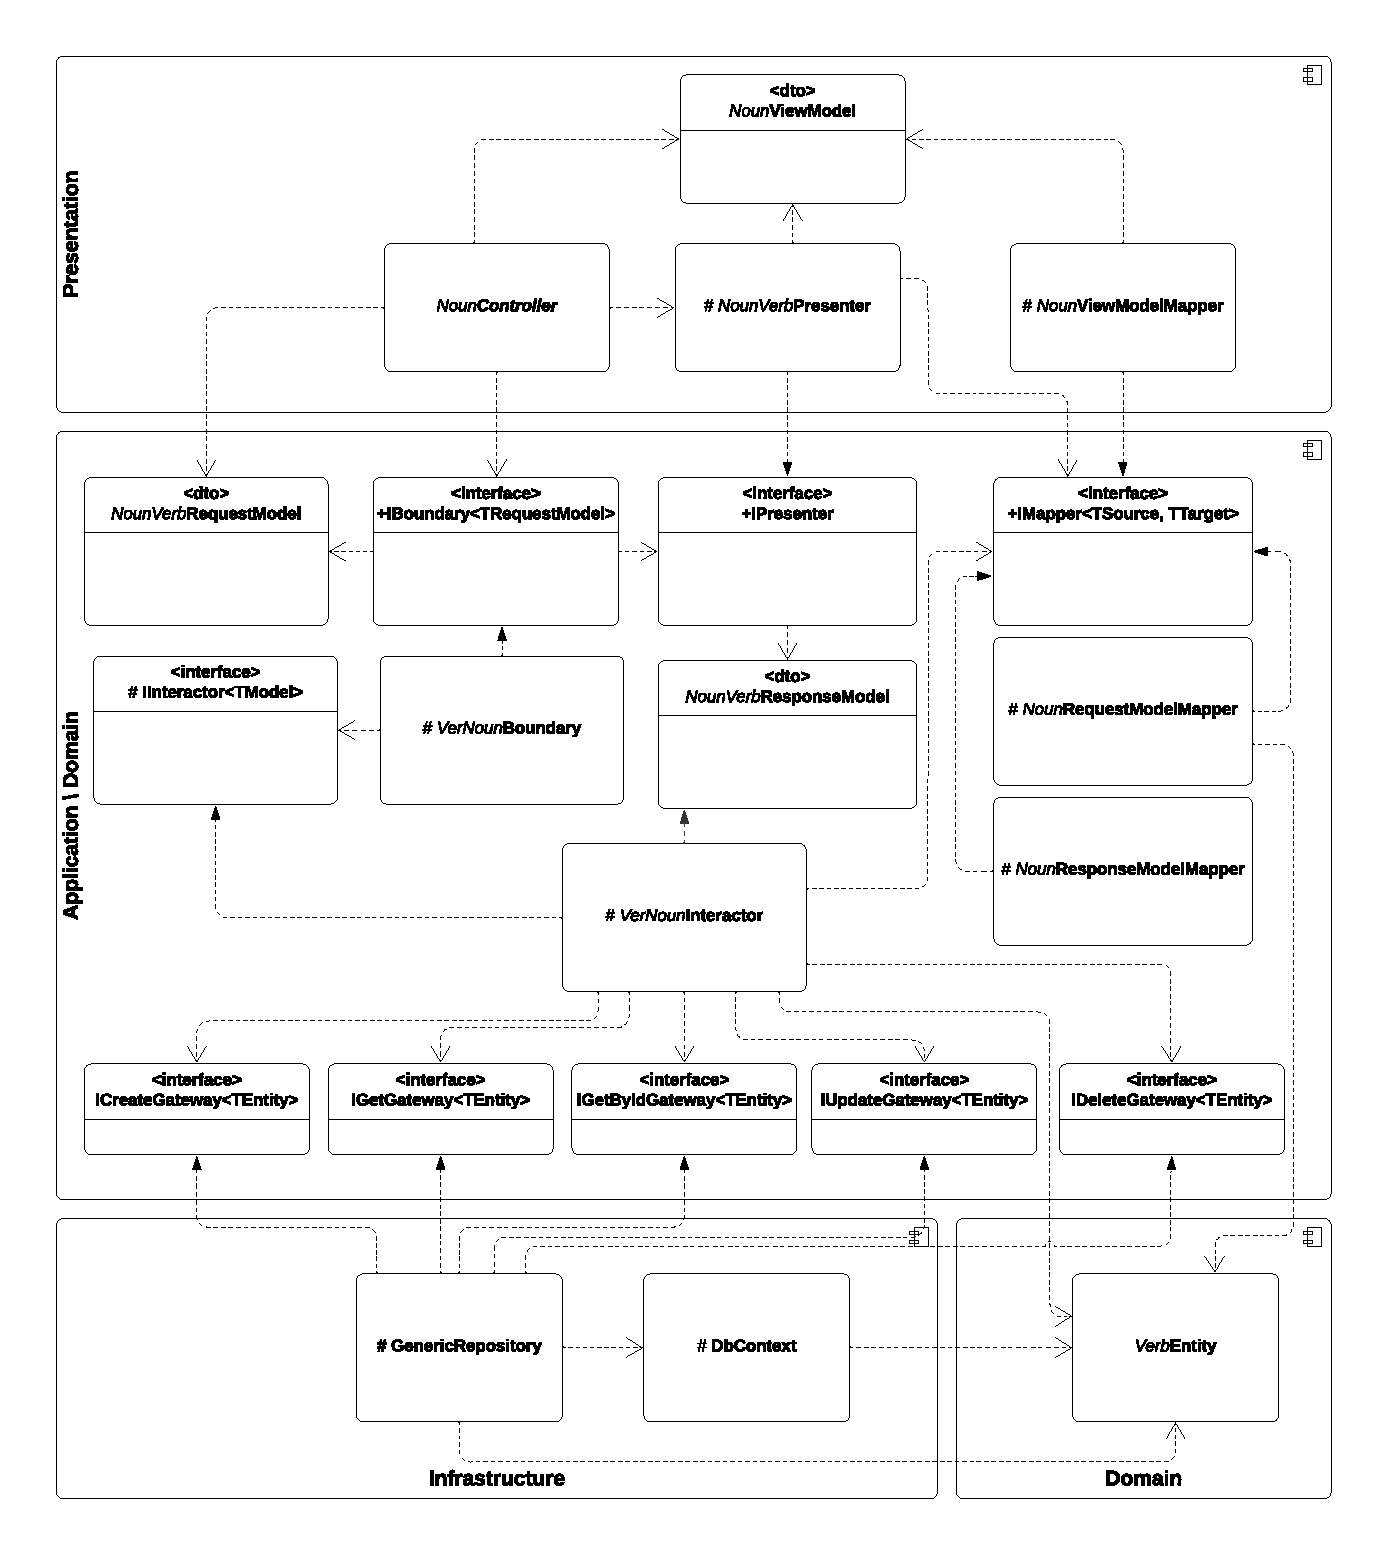
\includegraphics[width=\textwidth]{figures/generic_design.pdf}
    \caption[Generic architecture]{The Generic architecture of the artifacts}
    \label{fig_design}
\end{figure*}

The ViewModel consists of data attributes representing fields from the corresponding
Entity and may also contain information specific to the user interface. It is important to
note that the ViewModel has no external dependencies on other objects within the
architecture.

The Presenter is derived from the IPresenter interface and adheres to the specified
implementation, which is located in the Application layer. Its main responsibility is to
create the Controller's Response by instantiating the ViewModel, constructing the HTTP
Response message, or combining both as necessary. When needed, the Presenter utilizes the
IMapper interface without depending on specific implementations of IMapper. The Presenter
has an internal scope and cannot be instantiated outside the Presentation layer.

The ViewModelMapper, derived from the IMapper interface, follows the specified
implementation found in the Application layer. Its primary role is to map the necessary
data attributes from the ResponseModel to the ViewModel. The ViewModelMapper also has an
internal scope, ensuring it cannot be instantiated outside the Presentation layer.

The Controller is responsible for receiving external requests and forwarding them to the
appropriate Boundary within the Application layer. It relies on the IBoundary interface
without depending on specific implementations of this interface.

The IBoundary interface establishes the contract for its derived Boundary implementations,
and it has public scope within the system. Boundary implementations, derived from the
IBoundary interface, ensure separation between the internal aspects of the Application
Layer and the other layers. Each Boundary implementation handles a single task, executed
using the IInteractor interface. These implementations also have an internal scope and
cannot be instantiated outside the Application layer.

The IInteractor interface defines the contract for its derived Interactor implementations.
Like Boundary implementations, Interactors have an internal scope and are limited to the
Application layer. Interactor implementations execute single tasks or orchestrate a series
of tasks. Tasks dependent on infrastructure components, such as databases, are handled
through a Gateway. Additionally, Interactor implementations utilize the IMapper interface
to handle mapping between RequestModels, Entities, and ResponseModels.

The IMapper interface establishes the contract for Mapper implementations and has public
scope within the system. Derived from IMapper, the RequestModelMapper is responsible for
mapping the necessary data attributes from the RequestModel to an Entity. The
RequestModelMapper has internal scope and cannot be instantiated outside the Application
layer.

Similarly, the ResponseModelMapper is responsible for mapping data attributes from the
ResponseModel and follows the same implementation and scope restrictions as the
RequestModelMapper.

The IPresenter interface establishes the contract for Presenter implementations, typically
within the Presentation layer. It has public scope and ensures consistency in Presenter
behavior throughout the system.

The Gateway establishes the contract for interaction with infrastructure technologies such
as databases or filesystems. Each Gateway follows a specific naming convention, with
interfaces like ICreateGateway, IGetGateway, IGetByIdGateway, IUpdateGateway, and
IDeleteGateway representing different CRUD operations. Gateway implementations are derived
from these interfaces and are responsible for task-specific interactions with
infrastructure components. These implementations have internal scope and cannot be
instantiated outside their respective layers.

The ResponseModel consists of data attributes representing fields from the corresponding
Entity and may include output-specific data for the Interactor. The ResponseModel does not
depend on external objects within the architecture.

The RequestModel is similarly structured, consisting of data attributes from the
corresponding Entity and input-specific data for the Interactor. It, too, does not depend
on external objects within the architecture.

Data Entities represent corresponding data fields and do not rely on external objects.
They are only utilized by the Application layer.

The Gateway Implementation derives from the corresponding Gateway interface and adheres to
the specified implementation. It is responsible for handling tasks associated with its
infrastructure technology, such as interaction with a SQL database or filesystem. Gateway
Implementations have internal scope and cannot be instantiated outside their respective
layers.

Lastly, each architectural pattern adheres to at least one of the SOLID principles,
ensuring compliance and avoiding violations of these design principles.
